% Created 2022-01-26 Wed 17:58
% Intended LaTeX compiler: xelatex
\documentclass[11pt]{article}
\usepackage{graphicx}
\usepackage{grffile}
\usepackage{longtable}
\usepackage{wrapfig}
\usepackage{rotating}
\usepackage[normalem]{ulem}
\usepackage{amsmath}
\usepackage{textcomp}
\usepackage{amssymb}
\usepackage{capt-of}
\usepackage{hyperref}
\usepackage{abntex2cite}
\usepackage[T1]{fontenc}		% Selecao de codigos de fonte.
\usepackage[utf8]{inputenc}		% Codificacao do documento (conversão automática dos acentos)
\usepackage{microtype} 			% para melhorias de
\usepackage{xltxtra}
\usepackage{fontspec} %Font package
\newfontfamily\ch[Mapping=tex-text]{Noto Serif CJK TC}
\DeclareTextFontCommand{\unifont}{\ch}
\usepackage{xcolor} % to access the named colour LightGray
\definecolor{LightGray}{gray}{0.2}
\usepackage{minted}
\usemintedstyle{monokai}
\hypersetup{colorlinks, allcolors=., colorlinks=true, linkcolor={blue!78!white}, urlcolor={purple}, filecolor={winered}}
\usepackage{minted}
\usemintedstyle{monokai}
\graphicspath{../../}
\graphicspath{../../Resources/img/}
\author{Pedro G. Branquinho, Wei-Liang Qian (\ch{钱卫良})}
\date{17 December 2021}
\title{Simulation and Modeling of Traffic Congestion.}
\hypersetup{
 pdfauthor={Pedro G. Branquinho, Wei-Liang Qian (\ch{钱卫良})},
 pdftitle={Simulation and Modeling of Traffic Congestion.},
 pdfkeywords={},
 pdfsubject={},
 pdfcreator={Emacs 27.2 (Org mode 9.4.4)}, 
 pdflang={English}}
\begin{document}

\maketitle
\tableofcontents

\clearpage
\section{Abstract page}
\label{sec:org855d35c}
\subsection{Page for the Formulary Synthesis (§2)}
\label{sec:orgbde5ff5}

\begin{center}
\begin{tabular}{ll}
\hline
Name & Pedro Gomes Branquinho\\
USP Number & 9843240\\
Course & Engineer Physics\\
Enterprise Name & University of São Paulo\\
Enterprise Adress & Estrada municipal do Campinho, S/N, Campinho, Lorena/SP\\
Area of internship & Departamento de Ciências Básicas e Ambientais\\
Name of the Supervisor & Wei-Liang Qian (\ch{钱卫良})\\
Name of the Professor Supervisor & Luiz Tadeu Fernandes Eleno\\
Internship period & 01/10/2021 à 01/02/2022\\
Number of hours of Internship & 476h\\
\hline
\end{tabular}
\end{center}

\subsection{Page for the Enterprise Synthesis (§3)}
\label{sec:org2bef051}
\subsubsection{University of São Paulo (USP)}
\label{sec:orgde4e38d}
University of São Paulo is a public university. It's considered one of the
best one hundred universities in the world. Besides having excelence in the
formation of industrially oriented professionals, also USP is the greatest
Latin American university in terms of high quality publications.

\subsection{Description of the work (§4)}
\label{sec:org4e255dc}

We reproduced numerical method algorithms in this research. The initial
aim was at studying partial differential equations and to
recreate the simulations of a well known work on \emph{Traffic Flow}
\cite{kerner1993}. Although the end goal was not achieved, the
research provided knowledge on the topics of \emph{Numerical Stiffness} and
the limitations of \emph{Physics Informed Neural Network} (PINN).

\section{Introduction}
\label{sec:org56132cc}

Throughout the research, we used a \texttt{Version Control System} to keep a backup and
to track the progress; git and GitHub. The language chosen to model and compute
the PDEs was \texttt{Julia} \ref{sec:num-julia}.

The numerical methods explored consisted of Numerical
Analysis (von Neumman) \cite{press1986numerical}, Forward methods, and \texttt{Physics
Informed Neural Network} (PINN) \cite{zubov2021neuralpde}.

When the PINN method wasn't sufficient to solve the problem, a study about
\texttt{Numerical Stiffness} and the analytical numerical analysis became the focus of
the study. At this point, one of the programs developed dialed with simulating
\texttt{Stability Regions} of numerical methods.

The equations we intended to simulate are a \texttt{non-linear system} \ref{sec:non-linear}.

\subsection{Analytical standpoint}
\label{sec:org8baa5ab}
From a \emph{Analytical} point of view, Partial Differential Equations
(PDEs) differs from Ordinary Differential Equations (ODEs) in the
number of free variables. This means, in the case of PDEs the model depends on a
relationship of many variables and ODEs of only one.

\subsubsection{Definition}
\label{sec:orgf5b985d}
A \texttt{partial differential equation} means a relation, for a given function
\texttt{u(x,y,...)} \cite{john1978partial},
\begin{equation}
\label{eq:PDE}
\begin{aligned}
F(x,y,\ldots ,u,u_{x}, u_{y}, \ldots, u_{xx}, u_{xy}, \ldots{})=0
\end{aligned}
\end{equation}

If more than one partial differential equation is needed to describe a model,
then these PDEs are called a \texttt{system}.

If substituted an \(u(\mathbf{x})\) which satisfies
\(F(\mathbf{x},\mathbf{u(x)})=0\). Then, \texttt{u} is a solution of the \texttt{PDE} or the
\texttt{system}.

\subsection{Numerical standpoint}
\label{sec:org4836cc8}
The similarity between ODEs and PDEs, from a \emph{Numerical} point of view, is
that different approximation methods will result in different errors,
in relation to the exact, analytical, solution of the equations.

The need for numerical methods also unite both types of
equation. Since, even with ODEs as simple as the one derived from the
\emph{Simple Pendulum} do not have an analytical solution, without making simplifying
hypothesis \cite{brauer1989qualitative}.

\subsection{Methods studied}
\label{sec:org1601f68}

\subsubsection{Ordinary Differential Equation}
\label{sec:org50f4371}
Euler Forward, Backward and Adams-Moulton (trapezoidal) methods have been
studied with the standard test equation,

\begin{equation}
\begin{aligned}
y'(t)=e^{- \lambda{}t}
\end{aligned}
\end{equation}

This was done in other to both get used implementing numerical methods, and get
a better empirical sense of how different methods affect the accuracy of the
model.

Different variations of this system was simulated, in order to understand the
concepts of \texttt{Stiffness}, \texttt{A-stability} and \texttt{L-stability}.

\subsubsection{Nth-order methods for partial differentiation}
\label{sec:org719871a}
The numerical methods were further explored using the analytical derivation of
higher order numerical formulas. These derivations consisting in using Taylor
Series and arrive at a formula considering \texttt{n} points to calculate a step. E.g.,
for the second order partial differential of the third order

\begin{equation}
\begin{aligned}
\dfrac{\partial^2{u}}{\partial{x^2}}\biggr\rvert_i = \dfrac{u_{i+1}-2u_i+u_{i-1}}{\Delta{x^2}} - O(\Delta{x^2})
\end{aligned}
\end{equation}

\subsection{Analytical theory on perturbations}
\label{sec:org838b447}
On Kerner's paper, he uses perturbation theory to developed the analytical
formulas that implies the existence of a clustering effect - traffic jams - even
with extremely initial small perturbations \cite{kerner1993}.

In order to better understand these derivations, material has been studied on
the topic \cite{tremblay2017phy}, and a derivation of the spring-mass equations for a small pertubation
was derived.

\section{Bibliography Review}
\label{sec:orgeb24ab2}
\subsection{Development of the field}
\label{sec:orgcbdf3bb}
\subsubsection{The dawn of numerical methods}
\label{sec:org2e45f14}
Numerical analysis dawn can be dated to
1820 B.C. \cite{smith1930rhind}, with Egyptian's methods for
calculating roots.

Although, modern methods for solving ODEs and PDEs were mainly
developed after the discovery of \emph{Calculus}, in the 17th century.

\subsubsection{Modern methods and Computing}
\label{sec:org46fcfcf}
Currently, even though sophisticated mathematics has been
developed to accurately simulate virtually any ODE, the mathematics
for solving PDEs is still a open field. This is due to the nature of
PDEs which do not have a general method or procedure that is
efficient, when simulating them.

\subsubsection{Physics Informed Neural Networks}
\label{sec:org558bf63}
There exists methods aimed at using the computational power available in computers
to abstract the theoretical knowledge of Numerical Stability away from
the problem. \emph{Physics Informed Neural Network}
(PINN) is one of these methods. The shortcoming of the method is the loss of the
possibility of making small adjustments to the resulting \emph{Numerical
Method}, as will be discussed further on the results.

\subsubsection{Numerical Instability}
\label{sec:org0e0474f}
Each equation, and it's constant parameters, will have specific method
or a coupling of methods suited to the simulation of a PDE.

\subsubsection{Grouping of methods and types of PDEs}
\label{sec:org109f829}
Broadly, methods are associated with the kind of partial differential
equation one is studying. These equations can be either \texttt{Hyperbolic},
\texttt{Parabolic} or \texttt{Elliptic}. Also, equations can be mixed, e.g., \texttt{Mixed
Parabolic-Hyperbolic}, etc.

\subsection{Mathematical categorization of PDEs}
\label{sec:org26f9439}
\subsubsection{Order of equations and systems}
\label{sec:orgeaabdf4}
"The order of the system is the order of the highest derivative that occurs."
\cite{john1978partial}. In which, irrespective of the free variable, we count the
total number of derivatives. E.g., a sixth order equation, with mixed variables.

\begin{equation}
\label{eq:sixth-order}
\begin{aligned}
F(\mathbf{x},\mathbf{u(x)}) = 0 \, \land \,
F(\mathbf{x}) = \dfrac{\partial{}^6 \mathbf{u}}{(\partial{x})^2(\partial{y})^2(\partial{z})} + \dfrac{\partial^3{} \mathbf{u}}{(\partial{x})^3}
\end{aligned}
\end{equation}

\subsubsection{Linearity, quasi-linearity and non-linearity}
\label{sec:orgaa23f18}
\begin{enumerate}
\item Linearity
\label{sec:org1dda5ae}

Linearity is defined as not having any term in the \eqref{eq:PDE}, such that it's
a result of a multiplication of two independent terms. The independent terms
being \(\mathbf{x}\), \(u(\mathbf{x})\) and all partial derivatives of
\(u(\mathbf{x})\).

For example, the second order linear equation with constant
coefficients, \texttt{Kolmogorov's equation} \cite{evans1998partial},
\begin{equation}
\begin{aligned}
u_{t} - \sum_{i,j=1}^{n}{a^{ij}u_{x_{i}x_{j}}} + \sum_{i}^{n}{b^{i}u_{x_{i}}} = 0
\end{aligned}
\end{equation}

We see there is no non-linear terms, as the product \(u_{x_{i}}*u_{x_{j}}\), etc.

\item Non-linear equations
\label{sec:org6e5e11a}
\label{sec:non-linear}

The physical model we are interested deals with an equation similar to the
\texttt{Navier-Stokes} equation \cite{kerner1993}. The \texttt{Navier-Stokes} equations are a
nonlinear system \cite{john1978partial} \cite{kerner1993}.
E.i.,

\begin{equation}
\label{eq:NavEstEQ}
\begin{aligned}
\begin{cases}
&\mathbf{u}_t + \mathbf{u} \cdot{} D\mathbf{u} - \nabla \mathbf{u} = - Dp \\
&\text{div}(\mathbf{u}) = 0
\end{cases}
\end{aligned}
\end{equation}

\item Quasi-linear equations
\label{sec:org898f047}

A special kind of equations that follow under the category of non-linear
equations are the quasi-linear equations. These have the non-linear terms which
are of a lesser order than the order of the equation. E.g., the \texttt{Korteweg-de
Vries} equation \cite{john1978partial},

\begin{equation}
\begin{aligned}
u_t + c uu_{x} + u_{xxx} = 0
\end{aligned}
\end{equation}
\end{enumerate}

\subsubsection{Elliptic, hyperbolic and parabolic PDEs}
\label{sec:orgc786b13}
Given the general quasi-linear equation for a function \texttt{u},

\begin{equation}
\label{eq:general-2th-order}
\begin{aligned}
au_{xx} + 2bu_{xy} + cu_{yy} = d
\end{aligned}
\end{equation}

where \(a\), \(b\), \(c\) and \(d\) are of the form \(f(x,y,u,u_x,u_y)\).

We can develop an analysis of how the solution would behave. \emph{A priori}, the
solution \(\gamma\) is contained on the xy-plane.

From this consideration, if carried an analysis on the curve itself, we
ultimately arise at the condition:

\begin{equation}
\begin{aligned}
\dfrac{dy}{dx} = \dfrac{b \pm \sqrt{b^2 -ac}}{a}
\end{aligned}
\end{equation}

Then, if \(ac-b^2>0\) it's \texttt{elliptic}; else, if \(ac-b^2<0\) it's called
\texttt{hyperbolic}. Finally, if \(ac-b^2=0\) we call it \texttt{parabolic}.

These categories help understand the expected behavior of the solution. But, in
nonlinear cases the PDE do not characterize the solution behavior in these
categories; and in some linear cases, different regions will have different
types of behaviors, regarding the \texttt{elliptic}, \texttt{hyperbolic} and \texttt{parabolic}
characterization \cite{john1978partial}.

\subsection{Numerical Methods implemented in Julia}
\label{sec:org9a7ee03}
\label{sec:num-julia}

\subsubsection{The language}
\label{sec:org938bb15}
Julia was invented to be both highly performative and to be an unified general
purpose language. It's sophisticated, meaning the language has polymorphism
(\texttt{dispatches}), can be statistically of dynamically typed, has a powerful macro
system, and can function as an scripting language.

\subsubsection{PDEs}
\label{sec:orga87431a}
There exists a variety of libraries on \emph{numerical methods}
available in modern languages. Most of them with ports of libraries
written in C and FORTRAN. To list a few, from the \texttt{Julia}
documentation on available methods:

\begin{itemize}
\item General PDE approximation methods.
\item Transform methods.
\item Finite difference methods.
\item Finite element methods.
\item Finite volume methods.
\item Spectral element methods.
\item Boundary element, Boundary integral methods.
\item Mesh free methods and particle methods.
\item Virtual element methods.
\item Multi-method packages.
\item Non-classical methods.

\textbf{Source:} \url{https://github.com/JuliaPDE/SurveyofPDEPackages}
\end{itemize}
\subsection{PINN}
\label{sec:org6f2153b}
\label{sec:bib-PINN}

Physics Informed Neural Networks have different use cases. One of them is
scalability to higher dimensions. While standard methods can require a computing
power beyond current capability, Physics Informed Neural Networks only linearly
increase in use of memory, regarding dimensionality \cite{zubov2021neuralpde}.

Another use case, which fits our requirements, is the certainty of convergence
via the \textbf{Universal Approximation Theorem}. Specially, non-linear equation can be
approximated with physics informed neural networks \cite{raissi2019physics}.

\section{Materials and Methods}
\label{sec:org6eada4a}

The materials used were:
\begin{itemize}
\item Git
\item GitHub
\item Julia language
\item Org-mode
\end{itemize}

\texttt{Git} is a tool to manage versions of programs in the \texttt{GitHub} versioning
system. \texttt{Julia} is a high performance programming language. And, \texttt{Org-mode} is a
literate programming environment suited to computer programming research and
documentation.

\subsection{Version Control}
\label{sec:orgb168ce4}
The research was stored and gradually updated on GitHub, available at \url{https://github.com/BuddhiLW/wlq-carflow}. The structure of the root directory is the following:

\begin{minted}[frame=lines,fontsize=\scriptsize,linenos=false,bgcolor=LightGray]{shell}
tree ../.. -d -I "ltximg"
\end{minted}

\begin{figure}[!htb]
  \centering
  \caption{\label{fig:dir} }
  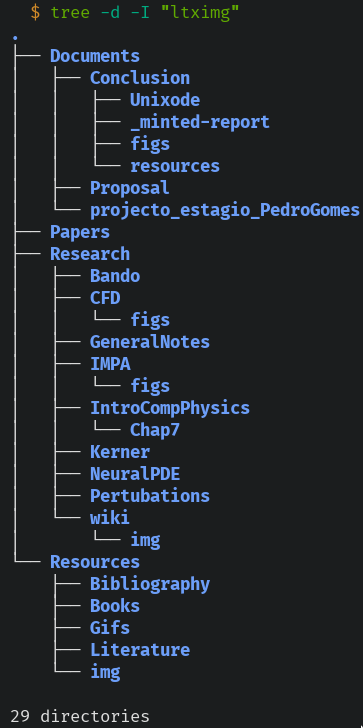
\includegraphics[width=0.45\linewidth]{Resources/img/directories.png}
  \legend{Source: The authors}
\end{figure}

This way, were able to document and keep track of the work, based on \texttt{Documents}, \texttt{Papers}, \texttt{Reseach} and \texttt{Resources}.

\subsection{Julia language}
\label{sec:orgc25f8ab}

Julia has been created by MIT personnel in order to fulfill segmented tasks
usually handled by different languages, in the process of \texttt{scientific
computing}. In our work, we used the libraries \texttt{NeuralPDE.jl}
\cite{zubov2021neuralpde}, and the native capabilities of Julia, to compute. To
plot graphics, we used both \texttt{GR} and \texttt{PyPlot} as out back-end for \texttt{Plots}.

\subsection{PINNs}
\label{sec:orgb9fe131}
The package \texttt{NeuralPDE.jl} has documentation on a variety of physical equations,
including non-linear equations and fluid equations. We used this package as a
means to reproduce the fluid equations in \texttt{Traffic Flow} modeling, as it's also
non-linear.

\texttt{NeuralPDE.jl} makes use of the \texttt{Symbolics.jl} and \texttt{ModelingToolkit.jl}
architecture. Therefore, our program structurally resembles the symbolical
notation used in mathematics.

\subsection{Developed code}
\label{sec:orge8a8007}
\label{sec:devcode}
As exercise to sharpen intuition about programs and physics computational
methods, simpler differential equations were solved. These were all done by
programs written by ourselves.

We used Euler Forward, Euler Backward, Trapezoidal Method, and a variety of
different point-approximations. These methods were tested in a category of
equations on exponential decayments.

\subsection{Stability Regions}
\label{sec:org50bcb78}
The stability region of a method is the region where, no matter the stepsize
used, the solution steadily converges to the real behavior. Therefore, the
accompanying plot for the simplified methods, discused in \ref{sec:devcode}, were
done, as well as the plot of the numerical method against the analytical solution.

\subsection{Pertubation theory}
\label{sec:orgd910530}
In the equations of motion of traffic jams, we need to understand pertubation
theory, so to understand how small pertubations will lead to singularities.

Therefore, as part of the research, we derived the pertubation equation for the
classical \texttt{mass-spring} problem.

\section{Results and Discussion (§5)}
\label{sec:orgfe7694b}
\subsection{Contribution to my formation}
\label{sec:orga89dadf}
\subsubsection{Technical knowledge}
\label{sec:orgc4360ac}
While many physics techniques were acquired, regarding the field of Applied
Numerical Methods, also I stayed in touch with all the programming required to
lead such a task. Therefore, I acquired knowledge on many subjects concerning
GNU/Linux systems, and programatically accessing the GPU with programming
languages.

Before the end of the period intended for this research, I received a proposal
for a job working with Linux and High Performance Computing (HPC). And, I can't
express enough how much the knowledge gathered using \texttt{Julia}, and staying in
touch with the scientific field has helped me. These two experiences heavily
impacted my interview for the Centro Nacional de Pesquisa em Energia e
Materiais (CNPEM).

\subsubsection{Self management}
\label{sec:orgfc96ccc}
One of the most difficult aspects of carrying on the research was the
motivational aspect. It's extremelly difficult to maintain a regular
performance, even more so when it's hard to even measure this performance
itself. While the quantity of content to be learned is infinite, one must learn
to direct it's energy and attention to topics that can be useful to the
research. Furthermore, the importante of knowing when to give up on a topic -  or
put the topic aside and replan the research - has been one of the most important
aspects of the research. Therefore, I learned to schedule and reschedule myself
dynamically and eval if I'm or not on track for my deadlines and objectives.

\subsection{Stiff equations}
\label{sec:org76b94b9}
We simulated the effects of stiffness in both \texttt{Ordinary Differential Equations}
(ODEs) and \texttt{Partial Differential Equations} (PDEs). The discussion in this
section will solemnly deal with notions concerning stiffness.

We will discuss the source of \emph{stiffness}, as there is no general definition for
the phenomena. Also, there is no mathematical formulation for it. Altough, the
concept arrises often, and was first discovered in an \texttt{Chemical Reaction}
modeling \cite{robertson1966solution}.

\subsubsection{Methods relly on using the \texttt{f} form}
\label{sec:org316c491}
As numerical methods, be them Euler, Trapezoidal etc., use the fact
that \(\dfrac{\partial{y_i}}{\partial{y_j}}=f_{ij}(y_1, y_2,
\ldots)\). Then, use the evaluation of \(f_{ij}\), in a discrete step
scheme, so to approximate the \(\mathbf{y}\) vector.

Therefore, mapping this mathematical formula \(f_{ij}\) to a programming
function can generalize the process and help to build many kinds of
"evolvers". Each method will have a general rule for writting an evolver,
because they appear out of analytical considerations on approximating functions.

Each different solver will have different error approximations. And some methods
may give rise to expurial behavior. Methods can be categorized as \emph{A-stable} or
\emph{L-stable}, depending on the caractheristics and behavior of the method regarding
a general model of a curve.

\subsubsection{Factors with high exponents}
\label{sec:org06878d1}
Even though a term may not greatly influence the analytical behavior of a
system, it may create the \emph{Stiffness} effect on numerical solvers.

For example, the Robert's equation

\begin{equation}
\begin{aligned}
{\dot {x}}=-0.04x+10^{4}y\cdot z
{\dot {y}}=0.04x-10^{4}y\cdot z-3\cdot 10^{7}y^{2}
{\dot {z}}=3\cdot 10^{7}y^{2}
\end{aligned}
\end{equation}

Have term with coefficients of order \(10^{-2},\,10^{4},\,10^{7}\). Even though
the main behaviour may be simply approximate to the terms of \(10^{7}\) order with
high precision, when we give a numerical solver to simulate the equation, it can
present expurious behavior due to this different order of coefficients. And,
given a simplified analytical equation, there would be neglectable expurious
behavior, for the same numerical methods.

\subsubsection{Example}
\label{sec:orgc19e7d9}
A very simple equation of decayment can show us what stiffness means.

\$y'(t)=-\(\lambda\)y(t),\quad t\(\ge\) 0,y(0)=1.\$

The exact solution, in orange, is

\(y(t)=e^{-\lambda{}t}\, with y(t)\to 0 as t\to \infty\).

\begin{figure}[!htb]
  \centering
  \caption{\label{fig:burguer-square} Decay equation with different numerical methods}
  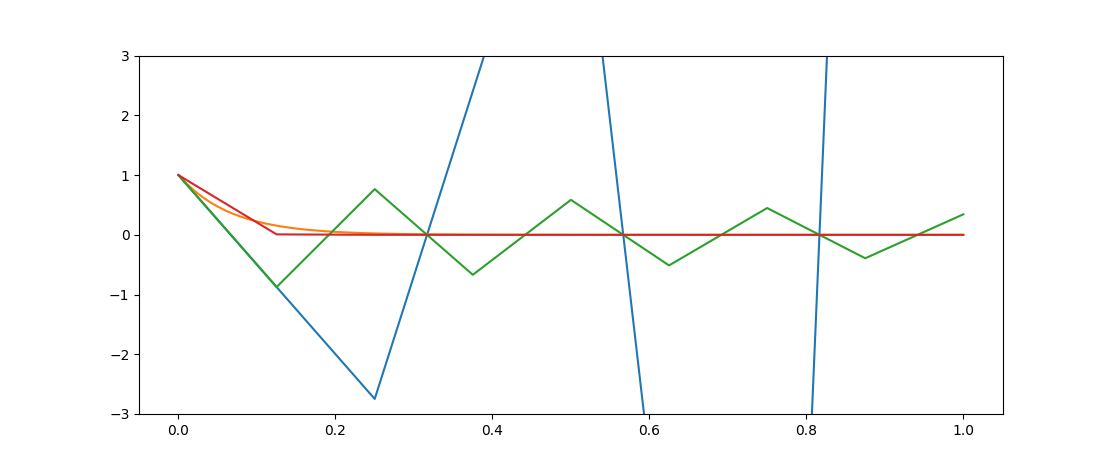
\includegraphics[width=0.70\linewidth]{Resources/img/Figure_2.png}
  \\  \legend{Source: the author. Red: Trap. (step=0.125); green: EuE (step=0.125); blue: EuE (step=0.25); orange: Analytical.}
\end{figure}

We see that Euler Explicit (EuE) gives us an unstable behavior. Increasing or
periodical, for the stepsizes of 0.25 and 0.125 respectivetly. In contrast, the
Trapezoidal method gives a quickly convergent approximation to the analytical
behavior.

For some special equations presenting \emph{Stiffness}, this expurious behavior is
present for almost all stepsizes and methods used - unless we use very small
stepsizes, which becomes computationally inefficient.

\subsection{Burguer 1-D with self-made program - Euler Explicit}
\label{sec:org8e946c7}

We solved the partial differential equation of non-linear conventionm
called Burguer's equation and described as,

$$\frac{\partial u}{\partial t} + u \frac{\partial u}{\partial x} =
0$$

\subsubsection{Mathematically, using Forward Euler}
\label{sec:orge2d8a08}

By Forward Euler,

$$\frac{u_i^{n+1}-u_i^n}{\Delta t} + u_i^n \frac{u_i^n-u_{i-1}^n}{\Delta x} = 0$$

$$u_i^{n+1} = u_i^n - u_i^n \frac{\Delta t}{\Delta x} (u_i^n - u_{i-1}^n)$$

\subsubsection{Computation in Julia}
\label{sec:org2e5b517}
\begin{enumerate}
\item Chose the discretization of \(x\) and \(t\)
\label{sec:orgc95adff}
\begin{minted}[frame=lines,fontsize=\scriptsize,linenos=false,bgcolor=LightGray]{julia}
nx=100;
# c=5;
delta_x = 40/(nx - 1)
x = range(0, stop=delta_x*(nx-1), length=nx) # full range of spatial steps for wich a solution is desired

endtime = 20   # simulation end time
nt = 1000          # nt is the number of timesteps we want to calculate
delta_t = endtime/nt  # δt is the amount of time each timestep covers
t = range(0, stop=endtime, length=nt) # full range of time steps for which a solution is desired
\end{minted}

\item Initial conditions
\label{sec:org6ef4665}
I have chose a square signal, as the initial condition
\begin{minted}[frame=lines,fontsize=\scriptsize,linenos=false,bgcolor=LightGray]{julia}
# Init array of ones at initial timestep
u_zero = ones(nx)

# Set u₀ = 2 in the interval 0.5 ≤ x ≤ 1 as per our I.C.s
u_zero[0.5 .<= x .<= 10] .= 2  # Note use of . (dot) broadcasting syntax
\end{minted}

\item Solving the equations
\label{sec:orgfc96bd8}
Create an empty matrix of the same size of the solutions we
intend. Then, we can solve utilizing various methods. But, we used
Euler Explicit for simplicity. 

\begin{minted}[frame=lines,fontsize=\scriptsize,linenos=false,bgcolor=LightGray]{julia}
u=zeros((nx,nt+1))
u[:,1]=copy(u_zero)

for n in 1:nt       # loop over timesteps, n: nt times
    u[:,n+1] = copy(u[:,n]) # copy the existing values of u^n into u^(n+1)
    for i in 2:nx 
	u[i,n+1] = u[i,n] - u[i,n] * delta_t/delta_x * (u[i,n] - u[i-1,n])
    end
end
\end{minted}

Then, finally, we can see how the equation evolves in time to a
wave-shaped equation, through \texttt{1-D Burguer's vicid} equation.
\begin{minted}[frame=lines,fontsize=\scriptsize,linenos=false,bgcolor=LightGray]{julia}
using Plots; pyplot()

xs = collect(x)
ts = collect(t)

plot(collect(x),collect(t),u'[1:1000,1:100],st=:surface, title="Burguer equation", xlabel="X", ylabel="Y", zlabel="U")
\end{minted}

\item Results
\label{sec:orgba78843}

When we use the \texttt{step function} and send it as an initial condition in the
burguer's equation. We see that the square equation becomes a bell-shaped
equation, evolving in time.

\begin{figure}[!htb]
  \centering
  \caption{\label{fig:burguer-square} Burguer's with square wave}
  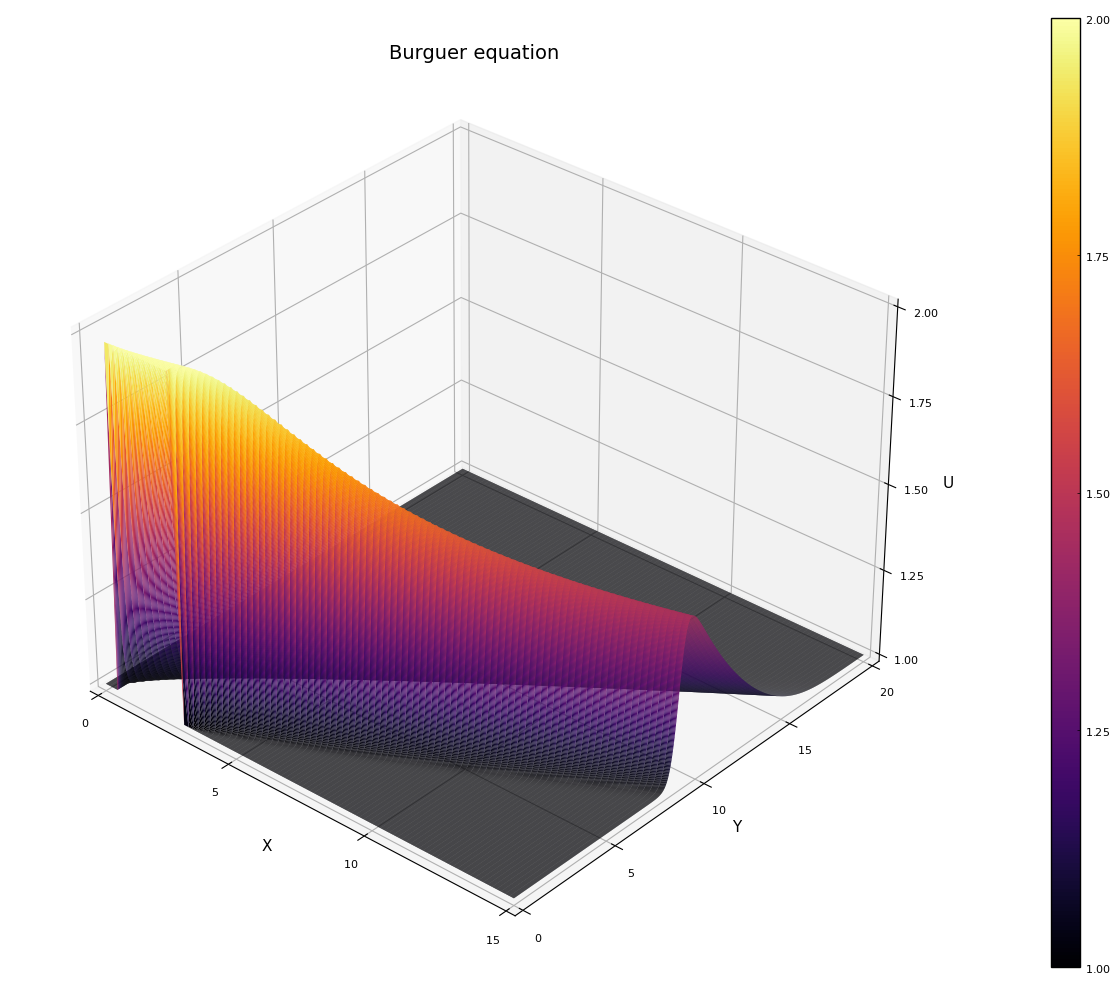
\includegraphics[width=0.45\linewidth]{Resources/img/Burguer.png}
  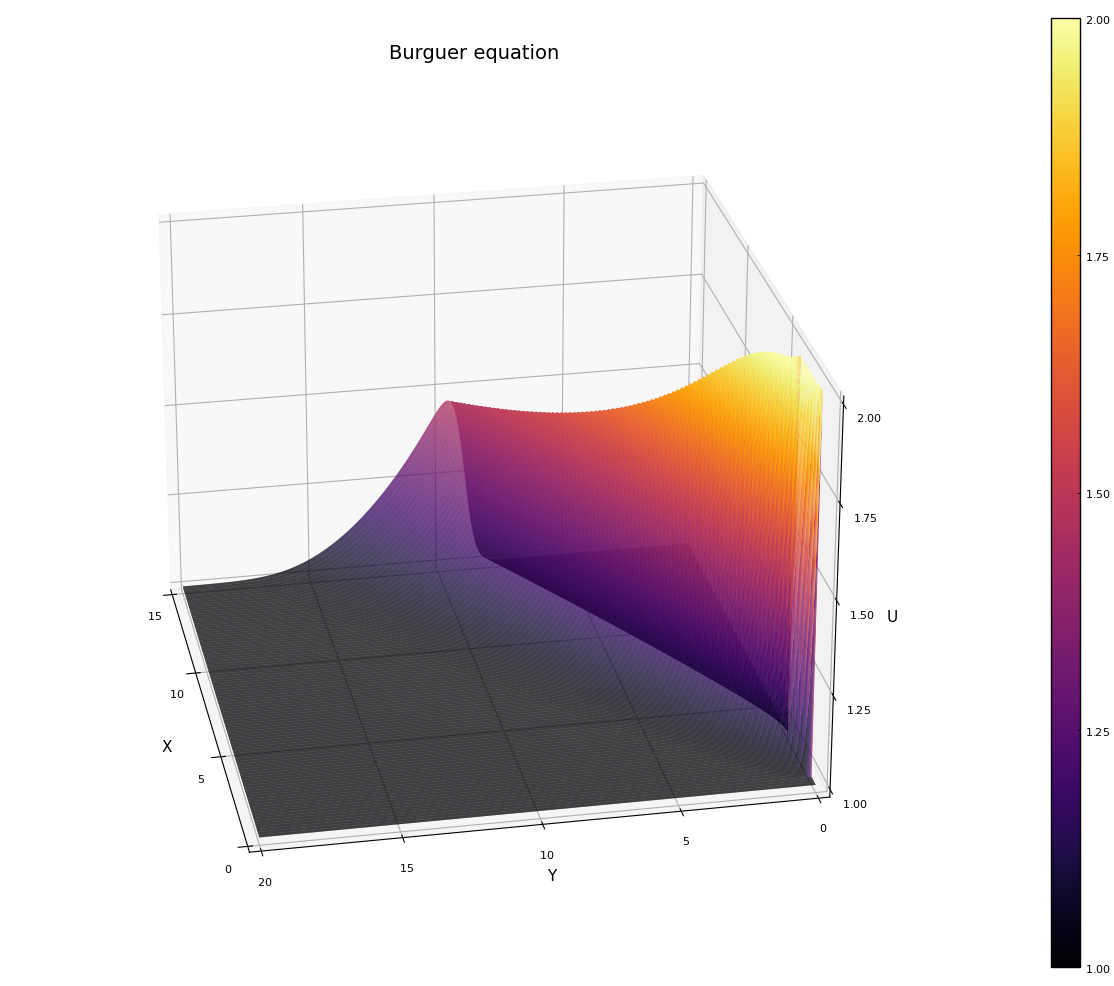
\includegraphics[width=0.45\linewidth]{Resources/img/Burguer2.png}
  \\  %\legend{Fonte: Imagem de Kerner e Konhäuser \cite{kerner1993cluster}}
\end{figure}

A step decrease in the function can be seen. This \texttt{dissipation} effecit is not found in
the equation. This is due to Euler Explicit method giving an exporious effect to
the solution. E.i., this is a numerical-error driven effect.

\begin{figure}[!htb]
  \centering
  \caption{\label{fig:burguer-square} Burguer's with square wave, views}
  \includegraphics[width=0.45\linewidth]{Resources/img/burguerNkerner/Burguer_32.png}
  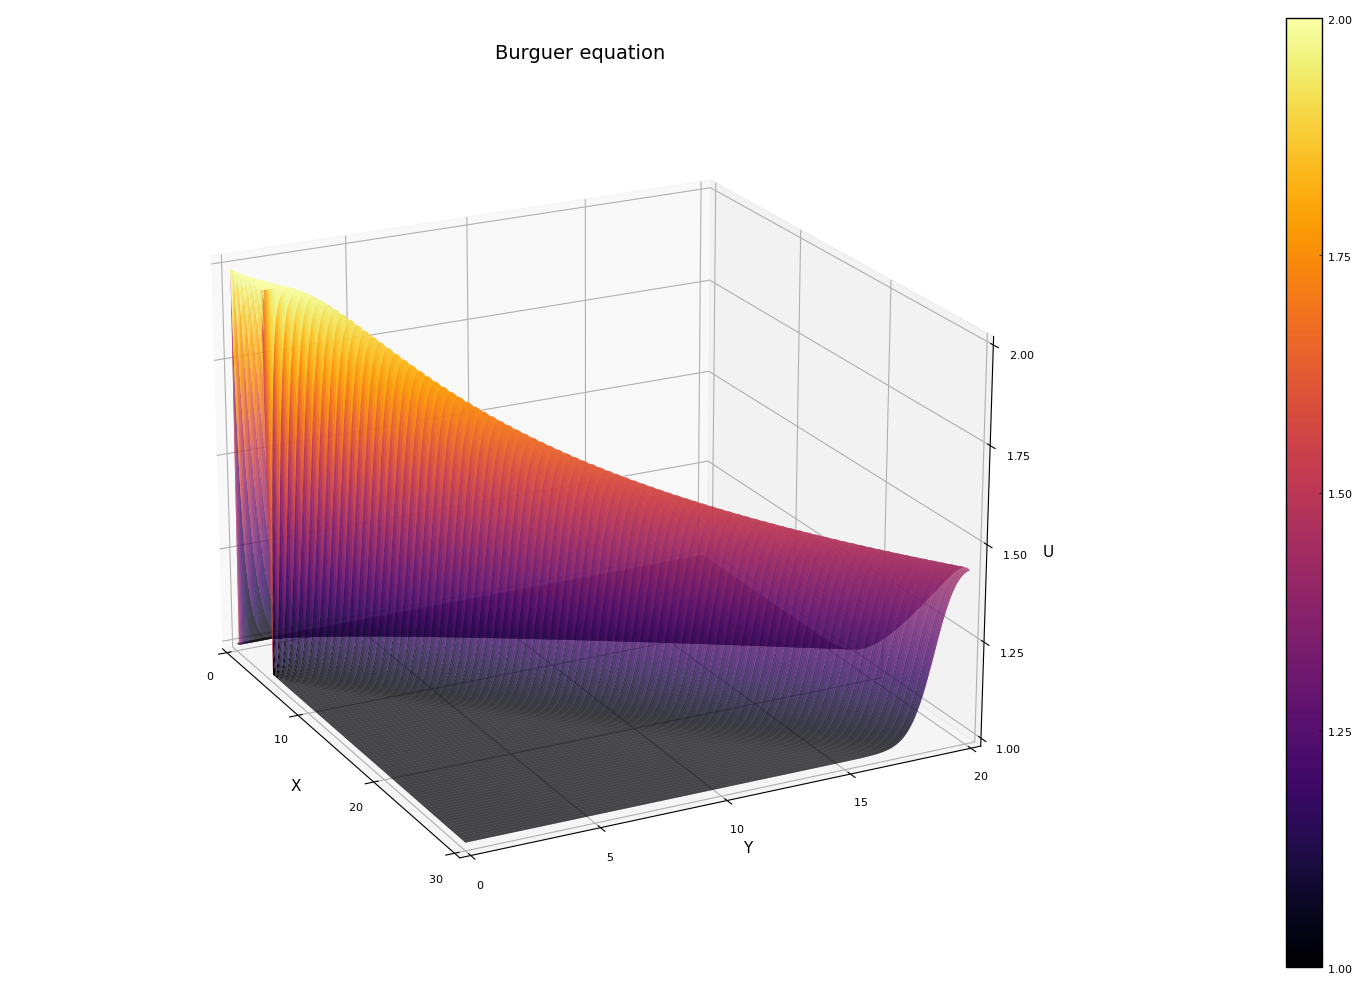
\includegraphics[width=0.45\linewidth]{Resources/img/Burguer_13.png}
  \\  %\legend{Fonte: Imagem de Kerner e Konhäuser \cite{kerner1993cluster}}
\end{figure}
\end{enumerate}

\subsection{Comparison: Analytical equation and Euler Explicit}
\label{sec:org7895e77}
\subsubsection{Computation}
\label{sec:org816223d}

We will utilize the same algorithm, with a different initial condition. This
time, we will use a normal wave, given by:

\begin{equation}
\begin{aligned}
f(x) = (\frac{1}{(2*\sqrt{\pi}))}*e^{[(\frac{-1}{2})*(x-3)^2]} \, \land \, u(t=0,x) = f(x) \\
\text{Domain: } x \in [0,10], \, t \in [0,20]
\end{aligned}
\end{equation}

The program, ajusting for f(x),

\begin{minted}[frame=lines,fontsize=\scriptsize,linenos=false,bgcolor=LightGray]{julia}
nxx=100;
delta_xx = 10/(nxx - 1)
xx = range(0, stop=delta_xx*(nxx-1), length=nxx) 

endTime = 20  
nt = 1000    
delta_t = endTime/nt  
t = range(0, stop=endTime, length=nt)

f(x) = (1/(2*√π))*exp((-1/2)*(x-3)^2)
v_zero = f.(xx) 

v_zero

v=zeros((nxx,nt+1))
v[:,1]=copy(v_zero)

for n in 1:nt  
    v[:,n+1] = copy(v[:,n]) 
    for i in 2:nxx  
	v[i,n+1] = v[i,n] - v[i,n] * delta_t/delta_xx * (v[i,n] - v[i-1,n])
    end
end

using Plots; pyplot()

xxs = collect(xx)
ts = collect(t)

plot(collect(xx),collect(t),v'[1:1000,1:100],st=:surface, title="Burguer equation Euler Explicit", xlabel="X", ylabel="Time", zlabel="V")
\end{minted}

\subsubsection{Analytical solution}
\label{sec:org228e512}
The solution to the Invicid Burguer Equation is:
\begin{equation}
\begin{aligned}
u(x,t) = f(x - f(\xi)t)
\end{aligned}
\end{equation}

in which \(f(x) = (\dfrac{1}{(2*\sqrt{\pi})})*e^{(-1/2)*(x-3)^2)}\), and \(\xi = 0\)
therefore, \(f(\xi)= (\dfrac{1}{(2*\sqrt{\pi})})*e^{(-1/2)*(-3)^2)}=0.003134\)

Finally, \(u(x,t)=f(x-0.00314t)\).

\begin{minted}[frame=lines,fontsize=\scriptsize,linenos=false,bgcolor=LightGray]{julia}
function u_real(x,t)
    return (1/(2*√π))*exp((-1/2)*((x-00314*t)-3)^2)
end
\end{minted}
\begin{minted}[frame=lines,fontsize=\scriptsize,linenos=false,bgcolor=LightGray]{julia}
u_real_val = map(z -> map(x -> u_real(x,z), xx), t)
\end{minted}

\begin{minted}[frame=lines,fontsize=\scriptsize,linenos=false,bgcolor=LightGray]{julia}
plot(collect(xx),collect(t),u_real_val,st=:surface, title="Burguer equation Analytical", xlabel="X", ylabel="Time", zlabel="V")
\end{minted}

\subsubsection{Comparison}
\label{sec:orga43a14a}

We see that both solutions shift to the right of the right axes with time, which
is expect. But, the numerical method based on \texttt{Euler Explicit} gives a
dissipation which is expurious. Furthermore, we see that the rate in which the
wave propagates the \texttt{x-axis} in time is increased by the \texttt{dissipative numerical
method}.

\begin{figure}[!htb]
  \centering
  \caption{\label{fig:burguer-square} Burguer's with square wave}
  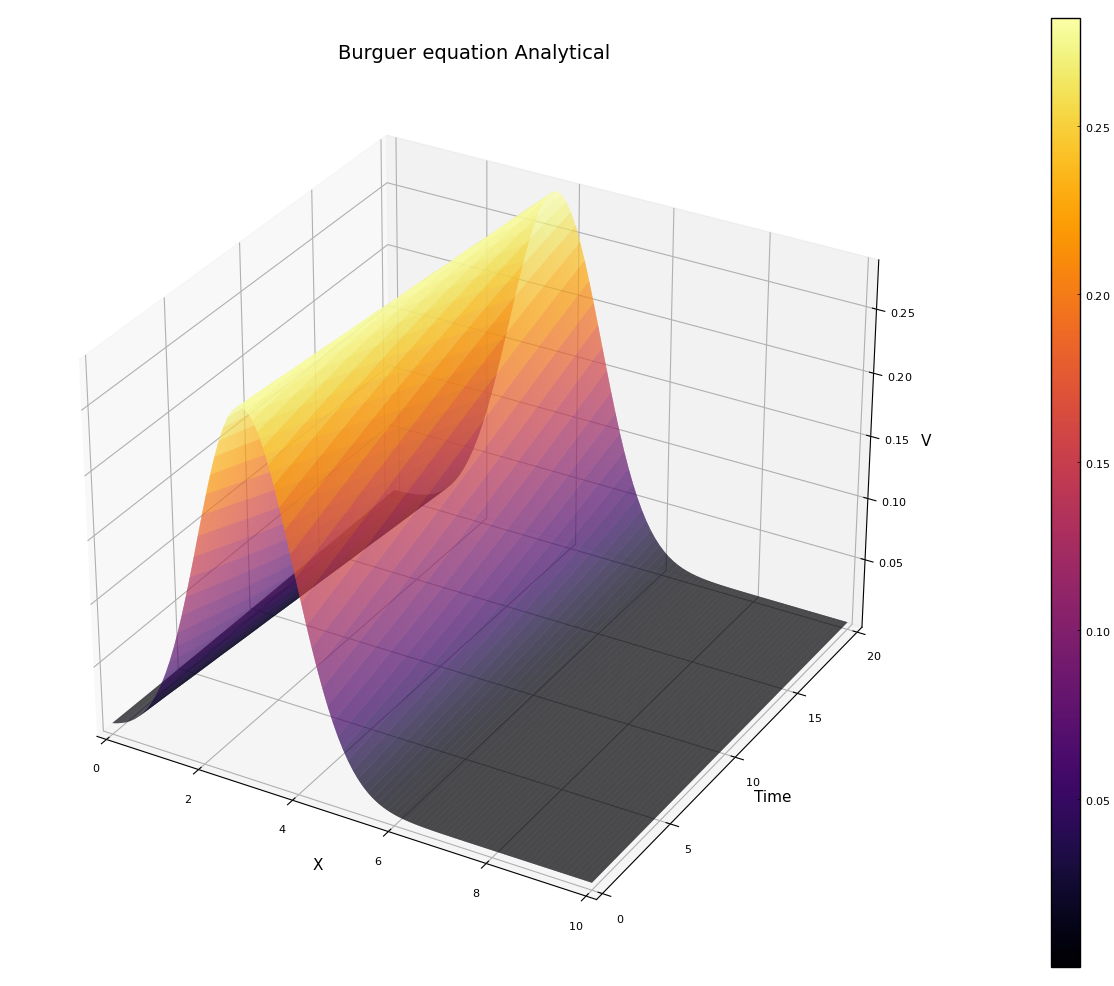
\includegraphics[width=0.45\linewidth]{Resources/img/BurguerAnalEuler/Burguer_Anal1.png}
  \includegraphics[width=0.45\linewidth]{Resources/img/BurguerAnalEuler/EulerExpicit_1.png}
  \\  %\legend{Fonte: Imagem de Kerner e Konhäuser \cite{kerner1993cluster}}
\end{figure}


This behaviour is equivalent to the expuriousness saw in the study of
\texttt{Stiffness}.

\subsection{Kerner's reproduction through PINNs}
\label{sec:org659aded}
\subsubsection{Mathematical description}
\label{sec:org8e302ee}
\begin{enumerate}
\item The System of Equations to solve
\label{sec:org68f1b41}
\begin{equation}
\begin{aligned}
\begin{cases}
\label{eq:NS-n1}
\left[\frac{\partial{v}}{\partial{t}} + v\frac{\partial{v}}{\partial{x}} \right] = \frac{1}{\rho{}}\dfrac{\partial \left(\mu \frac{\partial{v}}{\partial{x}} \right)}{\partial{x}} - \left(\frac{c_0^2}{\rho{}}\right)\dfrac{\partial{\rho}}{\partial{x}} + \frac{V(\rho) - v}{\tau} \\\\
     \dfrac{\partial{\rho}}{\partial{t}} + \dfrac{\partial{\left( \rho{}v \right)}}{\partial{x}}=0
\end{cases}
   \end{aligned}
 \end{equation}

\begin{equation}
\begin{aligned}
q(x,t)=\rho(x,t)v(x,t)
\end{aligned}
\end{equation}

\item Boundary Conditions
\label{sec:orgc4e6b75}
\begin{equation}
\begin{aligned}
q(0,t) &= q(L,t)\\
v(0,t) &= v(L,t),\quad \dfrac{\partial{v}}{\partial{x}}\biggr\rvert_0 = \dfrac{\partial{v}}{\partial{x}}\biggr\rvert_L
\end{aligned}
\end{equation}

From the definition of \(q\) and the boundary condition (I),
\begin{equation}
\begin{aligned}
&\rho(0,t)v(0,t) = \rho(L,t)v(L,t) \\
&\implies \rho(0,t) = \rho(L,t)
\end{aligned}
\end{equation}
\end{enumerate}

\subsubsection{The program}
\label{sec:org161d5a3}

We will use \texttt{NeuralPDE.jl} and other packages to model and optimize our
simulation. \texttt{ModelingToolkit.jl} makes possible to write our equations
symbolically; also, the boundary conditions. \texttt{GalaticOptim, Optim} are packages
to optimize the neural network approximations. \texttt{DiffEqFlux} makes possible to
partially derivate the symbolical equations.

\begin{enumerate}
\item Imports
\label{sec:org75211a0}
\begin{minted}[frame=lines,fontsize=\scriptsize,linenos=false,bgcolor=LightGray]{julia}
using NeuralPDE, Flux, ModelingToolkit, GalacticOptim, Optim, DiffEqFlux
import ModelingToolkit: Interval, infimum, supremum
import Flux: flatten, params
\end{minted}

\item The symbolical equations
\label{sec:orgb0e2c86}

Writting the equations following all constrains discussed in Section 1, in
Kerner's paper \cite{kerner1993},

\begin{minted}[frame=lines,fontsize=\scriptsize,linenos=false,bgcolor=LightGray]{julia}
@parameters t, x, N, L, ρ_hat, μ, c₀, τ, L, l,vₕ, k, m, ω, λ, γ
@variables v(..), ρ(..)
# ρ_hat=0.89;
m=1;
μ=1; #choose as we like
τ=1; #choose as we like
# l=sqrt(μ*τ/ρ_hat);

N = 10; # 168
ρₕ = 0.10; # 0.168
L=N/ρₕ;
δρ₀ = 0.02;
δv₀ = 0.01;
vₕ = 5.0461*((1+exp((ρₕ-0.25)/0.06))^-1 - 3.72*10^-6);

# vhat(ρ)= 5.0461*((1+exp((ρ-0.25)/0.06))^-1 - 3.72*10^-6);
# using Roots
# find_zero(vhat, (-5,5))
# 1.0001069901803379

# ρₕ=N/L;
k=2π/L;

c₀= 1.8634;
Dt = Differential(t)
Dx = Differential(x)
Dxx = Differential(x)^2

# δρₛ(x) = δρ₀*exp(complex(0,1)*k*x);
λ=(k^2*c₀^2)/100
ω=k*(vₕ+c₀)
γ=complex(λ,ω)

# δρ(t,x)=δρ₀*exp(complex(0,k*x))*exp(-γ*t)
# δv(t,x)=δv₀*exp(complex(0,k*x))*exp(-γ*t)

# Only real part
δρᵣ(t,x)=δρ₀*cos(k*x)*cos(ω*t)exp(-λ*t)
δvᵣ(t,x)=δv₀*cos(k*x)*cos(ω*t)exp(-λ*t)

#2D PDE
eqs  = [Dt(v(t,x)) + v(t,x)*Dx(v(t,x)) - (μ/ρ(t,x))*Dxx(v(t,x)) + (c₀^2/ρ(t,x))*Dx(ρ(t,x)) - (5.0461*((1 + exp(((ρ(t,x)-0.25)/0.06)))^-1 - 3.72*10^-2) - v(t,x))/τ ~ 0,
	Dt(ρ(t,x)) + Dx(ρ(t,x)*v(t,x)) ~ 0]
# Initial and boundary conditions
bcs = [ρ(t,0) ~ ρ(t,L),
       v(t,0) ~ v(t,L),
       Dx(v(t,0)) ~ Dx(v(t,L)),
       Dt(v(t,0)) ~ Dt(v(t,L)),
       ρ(0,x) ~ ρₕ + δρᵣ(0,x),
       v(0,x) ~ vₕ + δvᵣ(0,x)]

# Space and time domains
domains = [t ∈ Interval(0.0,1000.0),
	   x ∈ Interval(0.0,L)]
\end{minted}

\item Neural Network setup
\label{sec:orgd61ddd2}
Now, we choose how detailed we want the equations to be solved. This parameters
run a simulation that needs \textasciitilde{}5GB of RAM to save the resolution in memory.

\begin{minted}[frame=lines,fontsize=\scriptsize,linenos=false,bgcolor=LightGray]{julia}
# Neural network
input_ = length(domains)
n = 15
chain =[FastChain(FastDense(input_,n,Flux.σ),FastDense(n,n,Flux.σ),FastDense(n,1)) for _ in 1:2]
initθ = map(c -> Float64.(c), DiffEqFlux.initial_params.(chain))

_strategy = QuadratureTraining()
discretization = PhysicsInformedNN(chain, _strategy, init_params= initθ)

@named pde_system = PDESystem(eqs,bcs,domains,[t,x],[v(t,x),ρ(t,x)])
# @named pde_system = PDESystem(eqs,bcs,domains,[t,x],[u1(t, x),u2(t, x)])
prob = discretize(pde_system,discretization)
sym_prob = symbolic_discretize(pde_system,discretization)

pde_inner_loss_functions = prob.f.f.loss_function.pde_loss_function.pde_loss_functions.contents
bcs_inner_loss_functions = prob.f.f.loss_function.bcs_loss_function.bc_loss_functions.contents

cb = function (p,l)
    println("loss: ", l )
    println("pde_losses: ", map(l_ -> l_(p), pde_inner_loss_functions))
    println("bcs_losses: ", map(l_ -> l_(p), bcs_inner_loss_functions))
    return false
end
\end{minted}

\item Resolution computation
\label{sec:org79582cd}
\begin{minted}[frame=lines,fontsize=\scriptsize,linenos=false,bgcolor=LightGray]{julia}
res = GalacticOptim.solve(prob,BFGS(); cb = cb, maxiters=100) #5000
phi = discretization.phi

ts,xs = [infimum(d.domain):0.1:supremum(d.domain) for d in domains]

acum =  [0;accumulate(+, length.(initθ))]
sep = [acum[i]+1 : acum[i+1] for i in 1:length(acum)-1]
minimizers_ = [res.minimizer[s] for s in sep]
u_predict  = [[phi[i]([t,x],minimizers_[i])[1] for t in ts for x in xs] for i in 1:2]
\end{minted}

\item Plot 2D
\label{sec:orgc478cca}
Finally, we plot the solution in 2D,
\begin{minted}[frame=lines,fontsize=\scriptsize,linenos=false,bgcolor=LightGray]{julia}
# using Plots
using Plots
ts,xs = [infimum(d.domain):0.1:supremum(d.domain) for d in domains]

for i in 1:2
    p2 = plot(ts, xs, u_predict[i],linetype=:surface,title = "predict");
    plot(p2)
    savefig("sol_u$i")
end
\end{minted}

\item Plot 3D in time (Gif)
\label{sec:orgb08680b}

We reshape the output of the \texttt{res} variable (resolution) in a matrix form, such
we can plot it against each \texttt{t} and \texttt{x}.

\begin{minted}[frame=lines,fontsize=\scriptsize,linenos=false,bgcolor=LightGray]{julia}
prob = remake(prob,u0=res.minimizer)
res = GalacticOptim.solve(prob,ADAM(0.001);cb=cb,maxiters=2500)

phi = discretization.phi
ts,xs = [infimum(d.domain):0.1:supremum(d.domain) for d in domains]
u_predict = [first(Array(phi([t, x], res.minimizer))) for t in ts for x in xs]

using Printf

function plot_(res)
    # Animate
    anim = @animate for (i, t) in enumerate(0:0.05:t_max)
	@info "Animating frame $i..."
	u_predict_v = reshape([Array(phi([t, x, y], res.minimizer))[1] for x in xs for y in ys], length(xs), length(ys))
	u_predict_pho = reshape([Array(phi([t, x, y], res.minimizer))[2] for x in xs for y in ys], length(xs), length(ys))
	title = @sprintf("predict, t = %.3f", t)
	p1 = plot(xs, ys, u_predict_v,st=:surface, label="Velocity plot", title=title)
	title = @sprintf("real")
	p2 = plot(xs, ys, u_predict_pho,st=:surface, label="Density plot", title=title)
	plot(p1,p2)
    end
    gif(anim,"3pde.gif", fps=10)
end

plot_(res)
\end{minted}
\end{enumerate}

\subsubsection{Results}
\label{sec:org3543f28}
\begin{enumerate}
\item 2D Plots
\label{sec:orge00c713}

\begin{figure}[!htb]
  \centering
  \caption{\label{fig:sim1} Reproduction try, using PINN. Source: The authors}
  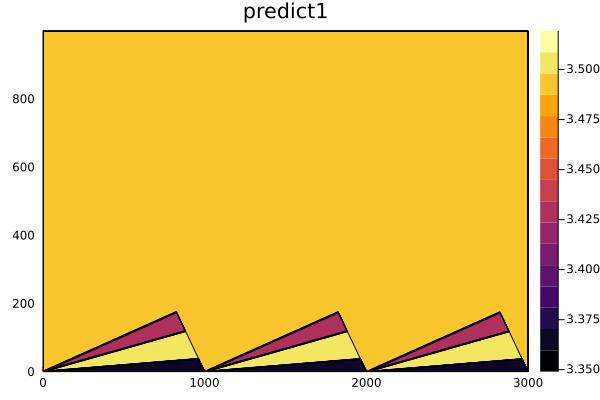
\includegraphics[width=0.45\linewidth]{Resources/img/sol_variable_corrected_bcs31.png}
  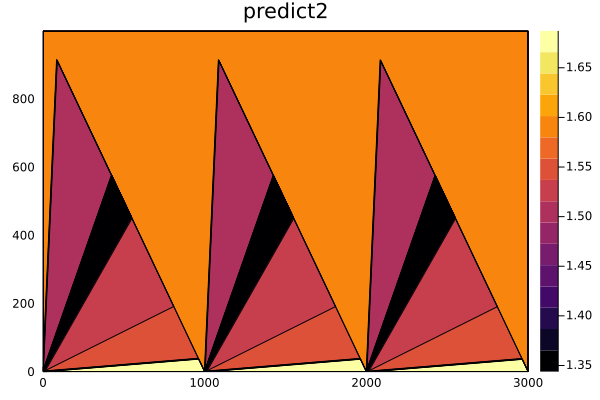
\includegraphics[width=0.45\linewidth]{Resources/img/sol_variable_corrected_bcs32.png}
  \\ %\legend{}
\end{figure}

\begin{figure}[!htb]
  \centering
  \caption{\label{fig:sim2} Original simulation. Source: Image from Kerner and Konhäuser \cite{kerner1993}}
  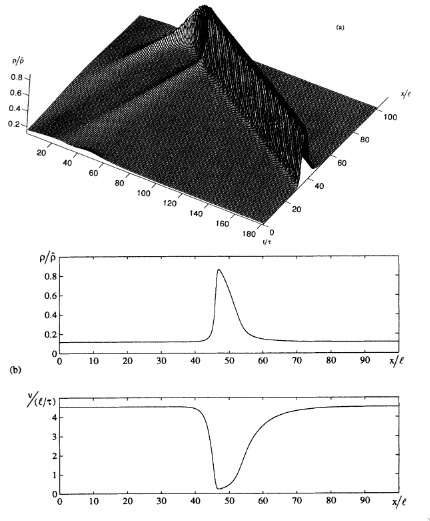
\includegraphics[width=0.4\linewidth]{Resources/img/kerner.png}
  \\  %\legend{Fonte: Imagem de Kerner e Konhäuser \cite{kerner1993cluster}}
\end{figure}

\item 3D Plots
\label{sec:orgfd4cd28}

\begin{figure}[!htb]
  \centering
  \caption{\label{fig:sim3} Representation of a time-cut of the PDE solution}
  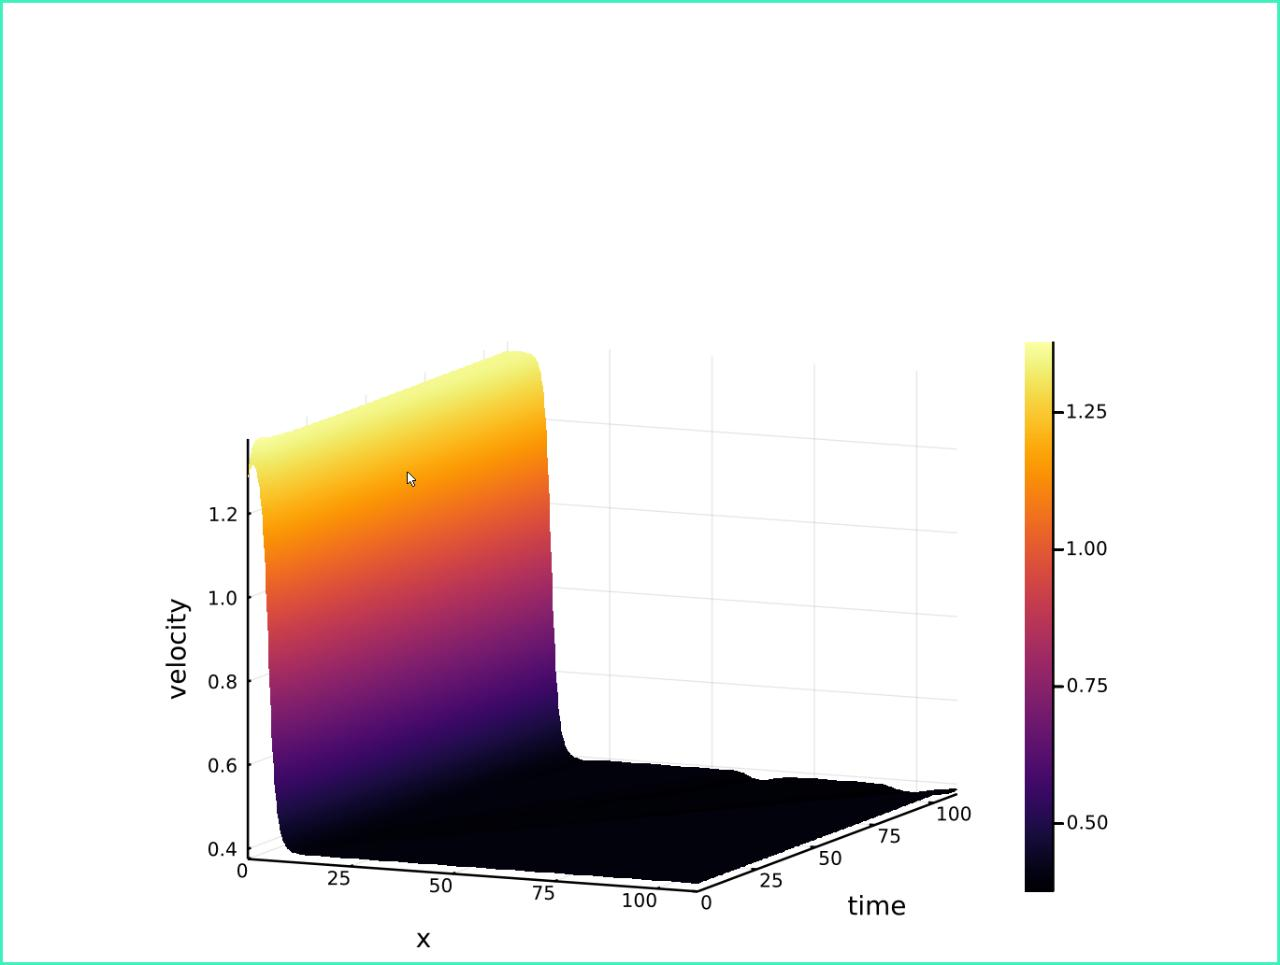
\includegraphics[width=0.45\linewidth]{Resources/img/Kerner-3d-1.jpeg}
  \\ \legend{Source: The authors}
\end{figure}

\begin{figure}[!htb]
  \centering
  \caption{\label{fig:sim3} Representation of a time-cut of the PDE solution}
  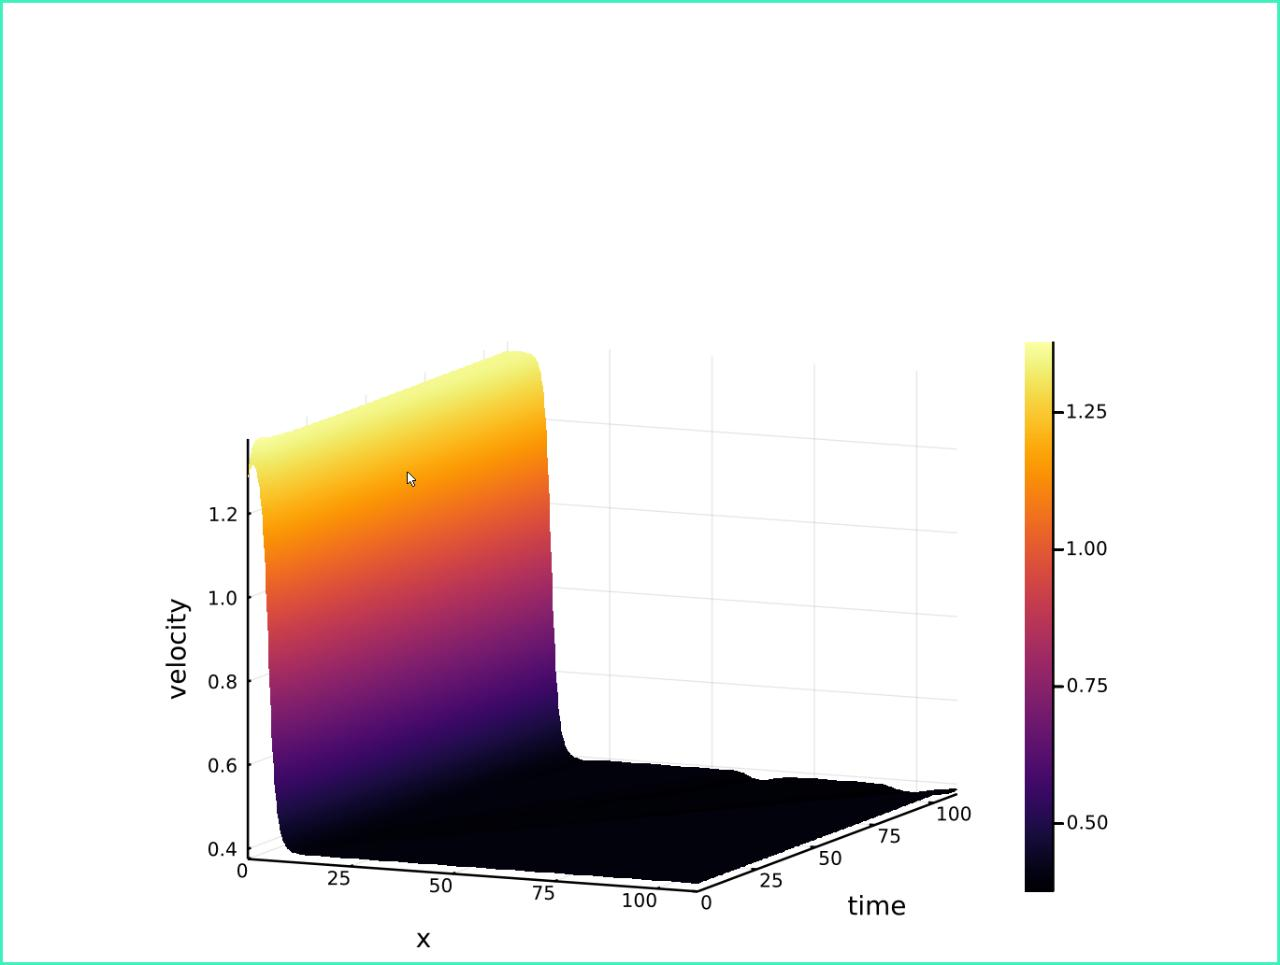
\includegraphics[width=0.45\linewidth]{Resources/img/Kerner-3d-1.jpeg}
  \\ \legend{Source: The authors}
\end{figure}

\begin{figure}[!htb]
  \centering
  \caption{\label{fig:sim4} PDE evolution in time, using PINN}
  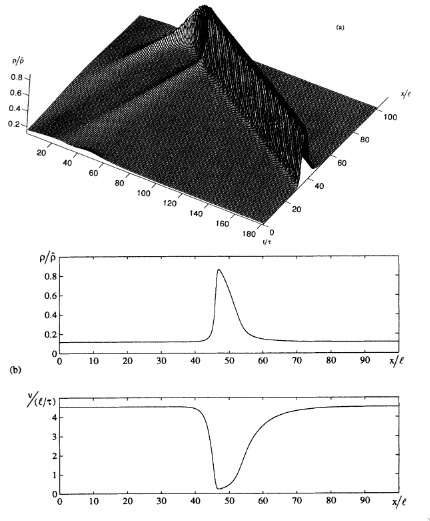
\includegraphics[width=0.4\linewidth]{Resources/img/kerner.png}
  \\ \legend{Source: The authors}
\end{figure}
\end{enumerate}

\subsection{Research on basic topics}
\label{sec:org2974ffe}
\subsubsection{Pertubation theory}
\label{sec:orgffea163}
The derivation of the pertubation of the \texttt{mass-spring} can be seen at
GitHub.

We depart from the equations of motion and power expansions,
\begin{equation}
\begin{aligned}
\ddot{q} &= f(q, \dot{q}) \, \land \,
\left(\ddot{q} = - \frac{k}{m}q \, \land \, f(q,\dot{q})= - \frac{k}{m}q \right{)}\\
\ddot{\rho} &= f(q_0, 0) + \rho \dfrac{\partial{f}}{\partial{\rho}}(q_0,0) + \dot{\rho} \dfrac{\partial{f}}{\partial{\dot{\rho}}}(q_0,0) \, \land \, \left( \rho = q - q_0 \right)
\end{aligned}
\end{equation}
Then, we arrive at
\begin{equation}
\begin{aligned}
\rho_0 &= (\sqrt{A^2 + B^2}) \cos{\left(\sqrt{\frac{k}{m}}t_0 - \alpha\right)},\, \\
 \text{in which,} \sin{(\alpha)} &= \dfrac{A}{\sqrt{A^2 + B^2}} \, \land \, \cos{(\alpha)}= \dfrac{B}{\sqrt{A^2 + B^2}}
\end{aligned}
\end{equation}

\begin{enumerate}
\item Where this knowledge is used in Traffic theory
\label{sec:org14c6700}
In Section 2, item \emph{B. Critical fluctuation}, Pertubation theory is used.

\begin{figure}[!htb]
  \centering
  \caption{\label{fig:perturbation} Pertubation derivation on Navier-Stokes equation}
  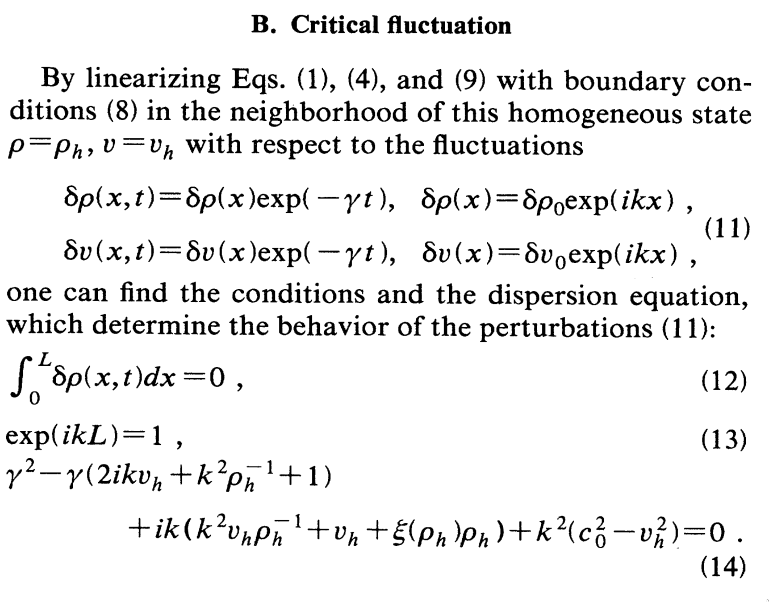
\includegraphics[width=0.45\linewidth]{Resources/img/kerner-pertubation.png}
  \\ %\legend{}
\end{figure}
\end{enumerate}

\subsubsection{Steps to derive the Stability Region}
\label{sec:org4200366}
\begin{enumerate}
\item Euler Implicit
\label{sec:orgb623d32}

From the definition of the method,
\begin{equation}
  \begin{aligned}
y_{n+1}&= y_n + \Delta{t}.f_n\\
\implies y_{n+1} &= y_{n} + \Delta{t}.\lambda{} y_{n}\\
\Leftrightarrow y_{n+1} &= y_{n}.(1+ \Delta{t}\lambda{}), \, \forall{n}\\
\implies y_n &= \left(1+ \Delta{t}\lambda{}\right)^n y_0
\end{aligned}
\end{equation}

So, we can derive, also given the step \texttt{n}, \(y_n\), we have \(y_{n+1}\). If the
\texttt{grow factor} is less than one, then the equation converges.

\begin{equation}
\begin{aligned}
y_{n+1} = y_n + \Delta{t}\lambda y_{n+1}\\
(1 - \Delta{t}\lambda{})y_{n+1} = y_n\\
y_{n+1} = \left(\dfrac{1}{1- \Delta{t} \lambda}\right) y_n
\end{aligned}
\end{equation}

Therefore, the stability region is given by,

\begin{equation}
\begin{aligned}
& \biggr\rvert\dfrac{1}{1- \Delta{t} \lambda} \biggr\rvert < 1 \\
\implies & |1 - \Delta{t} \lambda{}| > 1 \\
\Leftrightarrow & |z - 1| > 1
\end{aligned}
\end{equation}


Plotting the complex inequality, in \texttt{Julia},
\begin{minted}[frame=lines,fontsize=\scriptsize,linenos=false,bgcolor=LightGray]{julia}
f(a,b) = sqrt((a-1)^2 + b^2)
\end{minted}

\begin{minted}[frame=lines,fontsize=\scriptsize,linenos=false,bgcolor=LightGray]{julia}
plot(f ≫ 1, fill=(0,:blue))
\end{minted}

\begin{enumerate}
\item Plot of the stability region
\label{sec:orgdc9752d}
\begin{figure}[!htb]
  \centering
  \caption{\label{fig:stabEI} Stability region, Euler Implicit}
  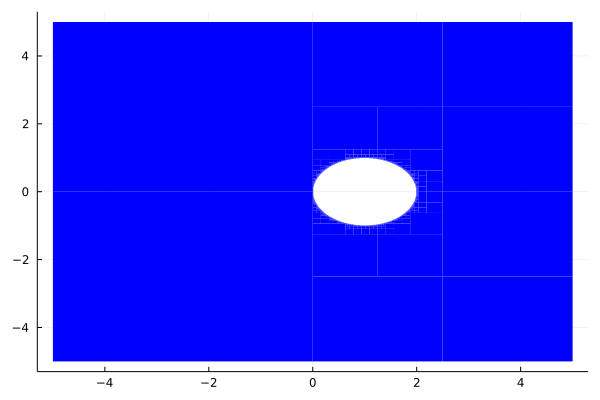
\includegraphics[width=0.45\linewidth]{Resources/img/curve2.png}
  \\ %\legend{}
\end{figure}
\end{enumerate}
\item Euler Explicit
\label{sec:orge6e63ff}

From the definition of the method,
\begin{equation}
  \begin{aligned}
y_{n+1}&= y_n + \Delta{t}.f_n\\
\implies y_{n+1} &= y_{n} + \Delta{t}.\lambda{} y_{n}\\
\Leftrightarrow y_{n+1} &= y_{n}.(1+ \Delta{t}\lambda{}), \, \forall{n}\\
\implies y_n &= \left(1+ \Delta{t}\lambda{}\right)^n y_0
\end{aligned}
\end{equation}

This model would only makes sense for \(|1+ \Delta{t} \lambda|<1, \,
\zeta(t) \in \mathbb{C}\).

Let \(z = \lambda{}\Delta{t}\), we can rewrite \(\zeta(t)\) as \(|z -
(-1)|<1\).

\begin{minted}[frame=lines,fontsize=\scriptsize,linenos=false,bgcolor=LightGray]{julia}
using ImplicitEquations, Plots
\end{minted}

\begin{minted}[frame=lines,fontsize=\scriptsize,linenos=false,bgcolor=LightGray]{julia}
f(a,b) = sqrt((a+1)^2 + b^2)
\end{minted}

\begin{minted}[frame=lines,fontsize=\scriptsize,linenos=false,bgcolor=LightGray]{julia}
plot(f ≪ 1, fill=(0,:blue))
\end{minted}

\begin{enumerate}
\item Plot of the stability region
\label{sec:orgffa2514}
\begin{figure}[!htb]
  \centering
  \caption{\label{fig:stabEI} Stability region, Euler Implicit}
  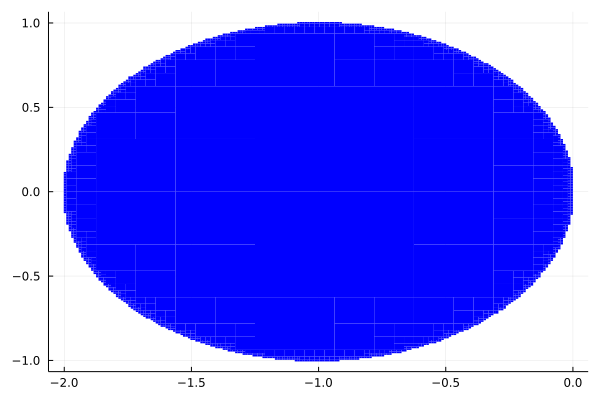
\includegraphics[width=0.45\linewidth]{Resources/img/curve.png}
  \\ %\legend{}
\end{figure}
\begin{enumerate}
\item PINN
\label{sec:orgafb5f91}
Via the Universal Approximation Theorem \ref{sec:bib-PINN}, Neural Networks have a
stability region that catches all the complex plane, in so far we choose enough
neural nets.
\end{enumerate}
\end{enumerate}
\end{enumerate}

\subsubsection{Stiffness}
\label{sec:org5dde9b8}
\begin{enumerate}
\item The stiff decayment equation (a particular example)
\label{sec:orgc285e15}
\begin{equation}
\begin{aligned}
x(t)=x_{0}\left(-{\frac {1}{999}}e^{-1000t}+{\frac {1000}{999}}e^{-t}\right)\approx x_{0}e^{-t}.
\end{aligned}
\end{equation}


So, that \(f(y,t) = x'(t) = x_0.(\frac{1000}{999}e^{-1000t} - \frac{1000}{999}e^{-t})\)

\item Numerical Methods
\label{sec:org6bfd6bf}
\begin{enumerate}
\item Euler Explicit (EuE), h=1/4
\label{sec:org2b13d14}
\begin{enumerate}
\item The method
\label{sec:orge058639}
\texttt{Euler Explicit}

\begin{equation}
\begin{aligned}
y_{n+1}&=y_n + \Delta{t}.f(y_n, t_n) \\
&= y_n + \Delta{t}.f_n
\end{aligned}
\end{equation}

\(\gamma\) will be your step functions.

\item \texttt{f} function
\label{sec:orgc0d9075}
\begin{minted}[frame=lines,fontsize=\scriptsize,linenos=false,bgcolor=LightGray]{julia}
function f₁(n, Δt,x₀=1.0)
    return x₀*((1000/999)*exp(-1000*n*Δt)-(1000/999)*exp(-n*Δt))
end

function f₁(n, Δt)
    return ((1000/999)*exp(-1000*n*Δt)-(1000/999)*exp(-n*Δt))
end
\end{minted}

\begin{verbatim}
f₁
\end{verbatim}

\item EuE implementation
\label{sec:org94c9077}
\begin{minted}[frame=lines,fontsize=\scriptsize,linenos=false,bgcolor=LightGray]{julia}
function EuE(y,f,n,Δt)
    return y[n] + Δt*f(y[n], n)
end
\end{minted}

\begin{verbatim}
EuE
\end{verbatim}

\begin{enumerate}
\item EuE step function
\label{sec:org9acaf11}
\begin{minted}[frame=lines,fontsize=\scriptsize,linenos=false,bgcolor=LightGray]{julia}
function γ₁(f, y::Vector{Float64}, Δt)
    yl = copy(y)

    push!(yl, EuE(y,f,length(y),Δt))

    return yl
end
\end{minted}

\begin{verbatim}
γ₁
\end{verbatim}

\item Initial condition
\label{sec:org0f2676e}
\begin{minted}[frame=lines,fontsize=\scriptsize,linenos=false,bgcolor=LightGray]{julia}
y₀=[1.]
\end{minted}

\begin{verbatim}
[1.0]
\end{verbatim}
\item Grid
\label{sec:org001147a}
\begin{minted}[frame=lines,fontsize=\scriptsize,linenos=false,bgcolor=LightGray]{julia}
tf = 1
Δt = 1/4
t = 0:Δt:tf
\end{minted}

\begin{verbatim}
0.0:0.25:1.0
\end{verbatim}

\item Step function test
\label{sec:orge2f6c55}
\begin{minted}[frame=lines,fontsize=\scriptsize,linenos=false,bgcolor=LightGray]{julia}
γ₁(f₁, y₀, Δt)
\end{minted}

\begin{verbatim}
[1.0, 0.9079380777849243]
\end{verbatim}


\begin{minted}[frame=lines,fontsize=\scriptsize,linenos=false,bgcolor=LightGray]{julia}
st1 = γ₁(f₁, y₀, Δt)
st2 = γ₁(f₁, st1, Δt)
γ₁(f₁, st2, Δt)
\end{minted}

\begin{verbatim}
[1.0, 0.9079380777849243, 0.8672235383623333, 0.8486675825957147]
\end{verbatim}
\end{enumerate}

\item Evolver
\label{sec:org12485da}
\begin{minted}[frame=lines,fontsize=\scriptsize,linenos=false,bgcolor=LightGray]{julia}
function evolveₖ(method, Δt, t_final=1.0, y₀=1.0, f=f₁)

    T = y₀
    t = 0.0

    ts = [t]
    results = [T]

    while t < t_final
	Tl = method(f,T,Δt) # new

	T = copy(Tl)
	push!(results, T)

	t += Δt
	push!(ts, t)
    end

    return ts, results
end

\end{minted}

\begin{verbatim}
evolveₖ
\end{verbatim}

\item Tests
\label{sec:orgde1ebc7}
\begin{enumerate}
\item Calling the Evolver
\label{sec:orga38b90c}
\begin{minted}[frame=lines,fontsize=\scriptsize,linenos=false,bgcolor=LightGray]{julia}
res = evolveₖ(γ₁, Δt, 10.0, y₀, f₁)
\end{minted}

\begin{verbatim}
Output suppressed (line too long)
\end{verbatim}
\end{enumerate}
\end{enumerate}

\item Euler Explicit (EuE), h=1/8
\label{sec:orga465418}
\begin{minted}[frame=lines,fontsize=\scriptsize,linenos=false,bgcolor=LightGray]{julia}
Δt = 1/8
\end{minted}

\begin{verbatim}
0.125
\end{verbatim}


\begin{minted}[frame=lines,fontsize=\scriptsize,linenos=false,bgcolor=LightGray]{julia}
res2 = evolveₖ(γ₁, Δt, 10.0, y₀, f₁)
\end{minted}

\begin{verbatim}
Output suppressed (line too long)
\end{verbatim}

\item Adams-Moulton, h=1/8 (Trapezoidal Method)
\label{sec:orgc4b95b2}
\begin{enumerate}
  \item The method
\label{sec:org316a53d}
\texttt{Trapezoidal}
\begin{equation}
\begin{aligned}
y_{n+1}&=y_n + \dfrac{1}{2}\Delta{t}.(f(y_n, t_n) + f(y_{n+1}, t_{n+1}))
\end{aligned}
\end{equation}
\item AM Evolver
\label{sec:orgf254161}
\begin{minted}[frame=lines,fontsize=\scriptsize,linenos=false,bgcolor=LightGray]{julia}
function AM(y,f,n,Δt)
    return y[n] + (1/2)*(Δt)*(f(n,Δt)+f(n+1,Δt))
end
\end{minted}

\begin{verbatim}
AM
\end{verbatim}

\item AM step function
\label{sec:org83db08f}
\begin{minted}[frame=lines,fontsize=\scriptsize,linenos=false,bgcolor=LightGray]{julia}
function γ₂(f, y::Vector{Float64}, Δt)
    yl = copy(y)

    push!(yl, AM(y,f,length(y),Δt))

    return yl
end
\end{minted}

\begin{verbatim}
γ₂
\end{verbatim}

\item Calling the Evolver
\label{sec:org6863662}
\begin{minted}[frame=lines,fontsize=\scriptsize,linenos=false,bgcolor=LightGray]{julia}
res3 = evolveₖ(γ₂, Δt, 10.0, y₀, f₁)
\end{minted}

\begin{verbatim}
Output suppressed (line too long)
\end{verbatim}
\end{enumerate}

\item Analytical
\label{sec:org7d2f946}
\begin{minted}[frame=lines,fontsize=\scriptsize,linenos=false,bgcolor=LightGray]{julia}
ts = 0:Δt:10
\end{minted}

\begin{verbatim}
0.0:0.25:10.0
\end{verbatim}


\begin{minted}[frame=lines,fontsize=\scriptsize,linenos=false,bgcolor=LightGray]{julia}
ys = ((-1/999)*exp.(-1000*t)+(1000/999)*exp.(-t))
\end{minted}

\begin{verbatim}
[1.0, 0.7795803634348398, 0.6071377975101436, 0.47283939213314785, 0.3682476888603027, 0.2867915884486388, 0.22335351366209194, 0.17394789134178695, 0.13547075399060332, 0.1055047292911555, 0.0821671657896885, 0.06399185305976735, 0.04983690527313708, 0.038813020852574584, 0.030227611033351854, 0.023541287143152262, 0.018333972861595774, 0.014278512421420678, 0.011120116654897204, 0.008660355558679314, 0.006744691690776244, 0.005252771170351737, 0.004090862300764832, 0.0031859667632729402, 0.0024812334100764353, 0.00193238652275046, 0.0015049441371146873, 0.001172051672463638, 0.0009127947603148311, 0.0007108852741166657, 0.0005536380081559896, 0.00043117371428997756, 0.0003357984263288407, 0.0002615200773790466, 0.00020367204105169588, 0.00015861994506081209, 0.00012353333742410368, 9.620785992131602e-5, 7.492675664434495e-5, 5.835301674761643e-5, 4.544537513762248e-5]
\end{verbatim}

\item Plots
\label{sec:orgdb08cc9}

Using \texttt{PyPlot.jl} backend,
\begin{minted}[frame=lines,fontsize=\scriptsize,linenos=false,bgcolor=LightGray]{julia}
pyplot()
\end{minted}

We create a figure on top of each other, for each simulation,
\begin{minted}[frame=lines,fontsize=\scriptsize,linenos=false,bgcolor=LightGray]{julia}
Plots.plot(res[1], res[2][length(res[2])], label="EuE 1/4")
\end{minted}

\begin{minted}[frame=lines,fontsize=\scriptsize,linenos=false,bgcolor=LightGray]{julia}
Plots.plot!(res2[1], res2[2][length(res2[2])], label="EuE 1/8")
\end{minted}

\begin{minted}[frame=lines,fontsize=\scriptsize,linenos=false,bgcolor=LightGray]{julia}
Plots.plot!(res3[1], res3[2][length(res3[2])], label="Trapezoidal 1/8")
\end{minted}

Finally, we plot the joing figure,
\begin{minted}[frame=lines,fontsize=\scriptsize,linenos=false,bgcolor=LightGray]{julia}
PyPlot.plot(ts,ys, label='Analytical')
\end{minted}

\item Result
\label{sec:orgfafb198}

We see that the Euler Explicit method fail to approximate the \emph{stiff equation}.
In comparison, the Trapezoidal Method lies on the stability region for the
approximation equation. Therefore, the behavior follows the analytical one

\begin{figure}[!htb]
  \centering
  \caption{\label{fig:sim1} Blue (EuE 1/4) and Orange (EuE 1/8); Green (AM 1/8); Purple (Analytical)}
  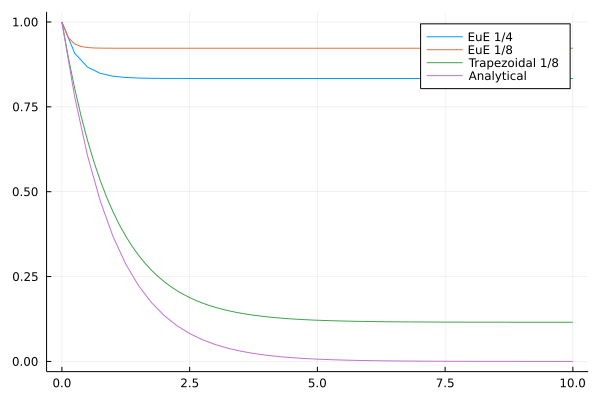
\includegraphics[width=0.45\linewidth]{Resources/img/exponential.png}
  \\ %\legend{}
\end{figure}
\end{enumerate}
\end{enumerate}

\subsubsection{Nth-order approximation}
\label{sec:org8c5ba0a}
Let \(u_i\) be the \texttt{i-th} node on our approximation grid. Then, we can create a
\emph{Taylor Expansion} forward and backwards, considering neighboring nodes, in order
to approximate a point-node.

\begin{enumerate}
\item Third-order approximation of second-order differential equation derivation
\label{sec:org5785936}
By \texttt{Taylor Expansion} on backwards expansion on \(u_{i+1}\) and forward on
\(u_{i-1}\), we can derive an expression for \(u_i\),
\begin{equation}
\begin{aligned}
\begin{cases}
u_{i+1} &= u_{i} + \Delta{x}\dfrac{\partial{u}}{\partial{x}}\biggr\rvert_i + \dfrac{\Delta{x^2}}{2!}\dfrac{\partial^2{u}}{\partial{x^2}} + \ldots \\
u_{i-1} &= u_{i} - \Delta{x}\dfrac{\partial{u}}{\partial{x}}\biggr\rvert_i + \dfrac{\Delta{x^2}}{2!}\dfrac{\partial^2{u}}{\partial{x^2}} + \ldots
\end{cases}\\
\sim
\begin{cases}
u_{i+1} &= u_{i} + \sum_{n=1}^{M}{\dfrac{(\Delta{x})^n}{n!}\dfrac{\partial^n{u(x)}}{\partial{x^n}}\biggr\rvert_i}\\
u_{i-1} &= u_{i} + \sum_{n=1}^{M}{(-1)^n\dfrac{(\Delta{x})^n}{n!}\dfrac{\partial^n{u(x)}}{\partial{x^n}}\biggr\rvert_i}
\end{cases}
\end{aligned}
\end{equation}

Summing both terms and isolating
\(\dfrac{\partial^2{u}}{\partial{x^2}}\biggr\rvert_i\), we have:

\begin{equation}
\begin{aligned}
\dfrac{\partial^2{u}}{\partial{x^2}}\biggr\rvert_i = \dfrac{u_{i+1}-2u_i+u_{i-1}}{\Delta{x^2}} - O(\Delta{x^2})
\end{aligned}
\end{equation}
\item Algorithm for Kerner's paper
\label{sec:org3d2b2d2}

Considering the general formula for each algorithmic step, we have,
\begin{minted}[frame=lines,fontsize=\scriptsize,linenos=false,bgcolor=LightGray]{julia}
wl[n]= w[n] + Δx*v[n]
ϕl[n]= ϕ[n] + Δx*ρ[n]
ρl[n] = ρ[n] - Δt*fρ(ρ,v,w,n)
vl[n] = v[n] - Δt*fv(ρ,v,w,Δx,n)
\end{minted}

In which, the five-point approximation for the \(f_{\rho}\) and \(f_v\) are,

\begin{minted}[frame=lines,fontsize=\scriptsize,linenos=false,bgcolor=LightGray]{julia}
function fρ(ρ,v,w,Δx,n)
    return (1/Δx)*(dif5_nt(ρ,n)*v[n]) + w[n]*ρ[n]
end
\end{minted}

\begin{minted}[frame=lines,fontsize=\scriptsize,linenos=false,bgcolor=LightGray]{julia}
function fv(ρ,v,w,Δx,n)
    return (1/Δx)*(v[n]*w[n]) + (μ/(ρ[n]*Δx))*(dif5_nt(w,n)) + (c₀^2/ρ[n]*Δx)*(dif5_nt(ρ,n)) + (1/τ)*(V(ρ[n])-v[n])
end
\end{minted}


Putting all in one \texttt{evolver-function},
\begin{minted}[frame=lines,fontsize=\scriptsize,linenos=false,bgcolor=LightGray]{julia}
function kerner(v::Vector{Float64},ρ::Vector{Float64},Δx,Δt,params,w=pbc_derivative(v,Δx),ϕ=pbc_derivative(ρ,Δx))
    N = length(v)
    vl=similar(v)
    ρl=similar(ρ)
    wl=similar(w)
    ϕl=similar(ϕ)
    μ, c₀, τ = params
    N = length(ρ)
    k=200π/1000
    δv₀ = 0.01
    δρ₀ = 0.02

    V(ρ) = 5.0461*((1+exp((ρ-0.25)/0.06))^-1 - 3.72*10^-6)

    for n in 2:N-1
	wl[n]= w[n] + Δx*v[n]
	ϕl[n]= ϕ[n] + Δx*ρ[n]
	ρl[n] = ρ[n] - (Δt/Δx)*(dif5_nt(ρ,n)*v[n]) + (Δt)*w[n]*ρ[n]
	vl[n] = v[n] - (Δt/Δx)*(v[n]*w[n]) + (μ*Δt/(ρ[n]*Δx))*(dif5_nt(w,n)) + (c₀^2*Δt/ρ[n]*Δx)*(dif5_nt(ρ,n)) + (Δt/τ)*(V(ρ[n])-v[n])
    end

    # Bondary condition
    ρₕ = 0.168
    vₕ = 5.0461*((1+exp((ρₕ-0.25)/0.06))^-1 - 3.72*10^-6)
    wl[N] = w[N] + Δx * v[N]
    ϕl[N] = ϕ[N] + Δx * ρ[N]
    ρl[N] = ρ[N] - (Δt/Δx)*((ρ[1]-ρ[N])*v[N] + w[N]*ρ[N])
    vl[N] = v[N] - (Δt/Δx)*(v[N]*w[N]) + (μ*Δt/(ρ[N]*Δx))*(w[1]-w[N]) + (c₀^2*Δt/ρ[N]*Δx)*(ρ[1]-ρ[N]) + (Δt/τ)*(V(ρ[N])-v[N])

    ϕl[1] = 0
    ϕl[length(ϕl)] = ρₕ*L
    ρl[1] = ρl[N]
    vl[1] = vl[N]
    return vl, ρl, wl, ϕl
end
\end{minted}
\end{enumerate}

\subsubsection{A-stable and L-stable}
\label{sec:org32c6307}
\begin{enumerate}
\item A-stable
\label{sec:org46b86b8}

\begin{quote}
The solution of this equation is \(y(t) = e^{kt}\). This solution
approaches zero as \(t\to \infty\)  when  \(\mathrm {Re} \,(k)<0\). If the
numerical method also exhibits this behaviour (for a fixed step size),
then the method is said to be A-stable.
\end{quote}

\texttt{A-stable} methods are those who are coherent with the general
behaviour of a function.

Not necessarily converges fast, or accurately. But, goes to the right
values over large times.

\item L-stable
\label{sec:org2ea34a4}
\texttt{A-stable} and the growth-factor goes to zero, as z goes to infinity
(converges even for really large steps). Therefore, \texttt{L-stability} is more
restrict than \texttt{A-stability}. L-stable methods are, necessarily, A-stable.
\end{enumerate}

\section{Conclusion (§6)}
\label{sec:orgfaa285c}
The use of PINNs got us closer to reproducing Kerner's
results. But, at the same time, the pigtail of using a method. This method
hide us the ability of adjusting the discretization. Once the results were not
satisfactory and there were no insight on where we may improve the computational
method.

After getting stuck on this riddle, we took the path of learning more
about \emph{classical methods} on numerical methods for PDEs. Knowledge on
the subject of \emph{equation Stiffness} was gained in the process e.g., why
and how to categorize methods and to grasp what does it mean to an
equation to be stiff.

The computations made in this work were: a diversity of tries regarding equation-parameters on
Navier-Stoker's equation; we also programmed a program to solve the 1D-Burguer's
equation successfully. A program has began to be develop that use Classical
Methods to solve Kerner's equation, which consisted in a five-point
approximation on space and a back-wards approximation on time.

\bibliography{../../../../Bibliography/collection}
\end{document}
